\begin{figure}[!htbp]
\centering
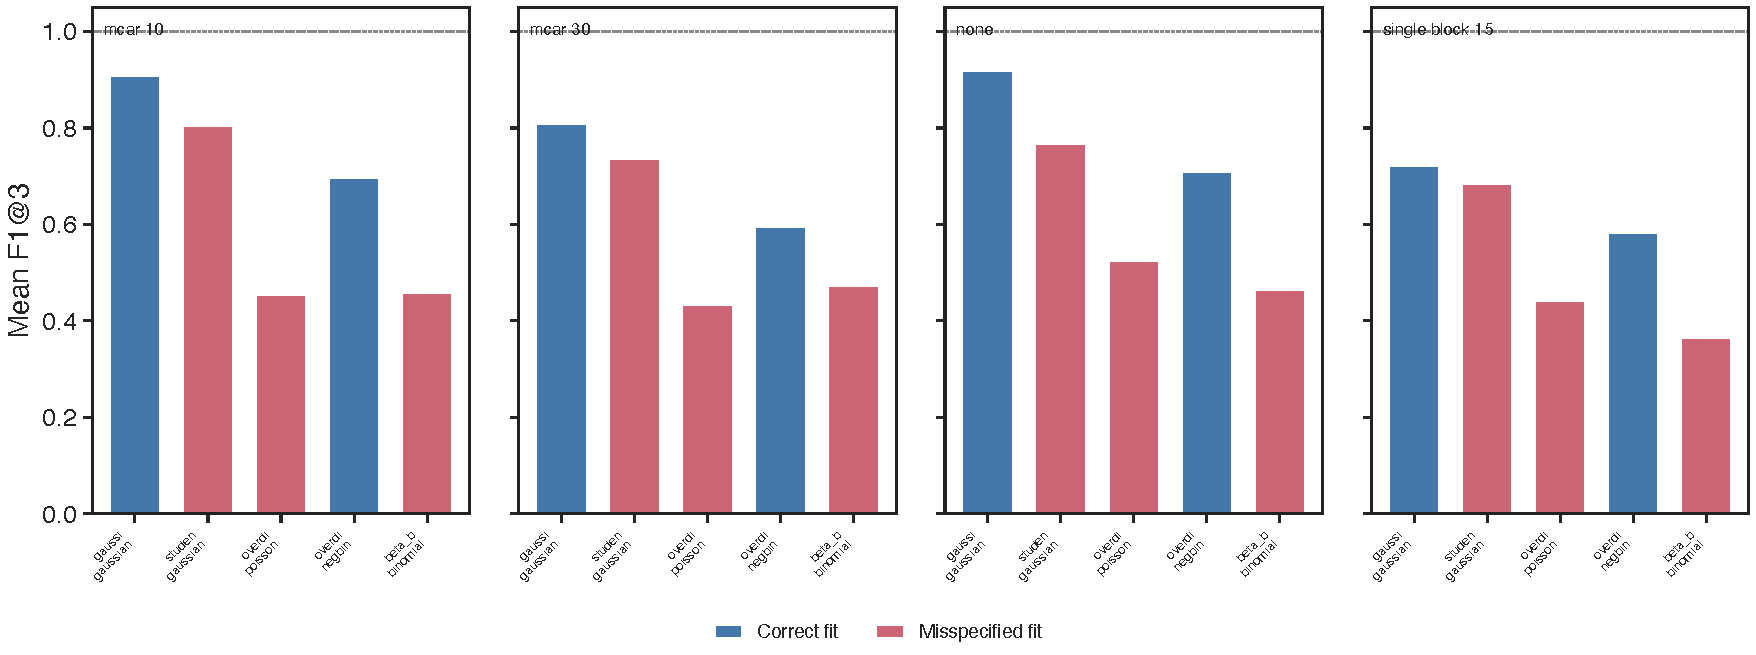
\includegraphics[width=0.98\linewidth]{shared/figures/results/fig_E07_robustness.pdf}
\caption{E07 misspecification and missing data: mean MAP boundary $\mathrm{F}_1@3$
by data-generating family (rows within each panel) and missingness condition (columns).
Blue bars: correctly specified fits; coral bars: misspecified fits.
Gaussian reference with correct Gaussian fit (blue) provides the baseline.
Student $t_3$ data fit by Gaussian (coral) shows moderate degradation.
NegBin data fit by Poisson (coral) shows larger degradation; the correct NegBin fit
(blue) recovers substantially higher accuracy.
Beta-Binomial data fit by Binomial (coral) shows the largest degradation:
overdispersion inflates the apparent segment count.
All 2000 replicates (20 cells $\times$ 100 each) completed with no numerical failures.
}
\label{fig:planned-robustness-paper}
\end{figure}
